\newpage

\section{Reti Bayesiane}

Sono dei modelli utili in situazioni di \textbf{incertezza}.\\

\textbf{Esempio}

Si modella la seguente situazione\dots

\begin{itemize}
\item L'allarme di casa (\textbf{A}) può scattare a causa di un terremoto (\textbf{E})
\item L'allarme di casa (\textbf{A}) può scattare a causa di un'intrusione (\textbf{B})
\item L'allarme di casa (\textbf{A}) acceso può portare Mary (\textbf{M}) o John (\textbf{J}) a chiamarmi
\end{itemize}

Le variabili del problema sono state riportate fra parentesi in grassetto: A, E, B, M, J.
La rete bayesiana che rappresenta la situazione è rappresentata in figura \ref{fig:alarm}:

\begin{figure}[H]
\centering
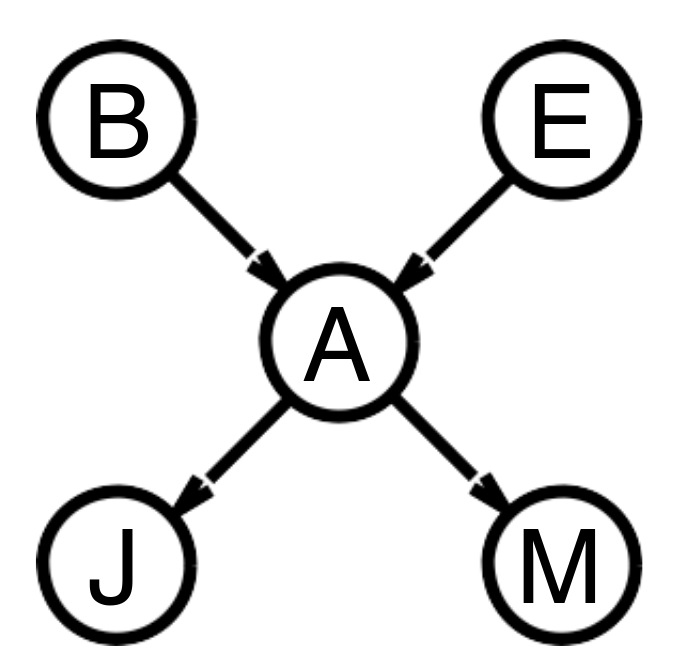
\includegraphics[width=0.25\textwidth]{alarm}
\caption{Rete bayesiana che modella l'esempio precedente}
\label{fig:alarm}
\end{figure}

Gli archi rappresentano le \textbf{dipendenze} tra le variabili (nodi): $X \rightarrow Y$ significa che X influenza direttamente Y.

Una rete bayesiana è un \textbf{grafo orientato senza cicli}.

Ciascun nodo/variabile/evento ha una certa probabilità di verificarsi, data la probabilità dei suoi genitori.

Questa viene detta probabilità condizionata ed è rappresentata tramite delle tabelle di distribuzione di probabilità condizionata \textbf{CPT}. Nell'immagine \ref{fig:cpt} le CPT vengono associate ai nodi della rete bayesiana dell'esempio:

\begin{figure}[H]
\centering
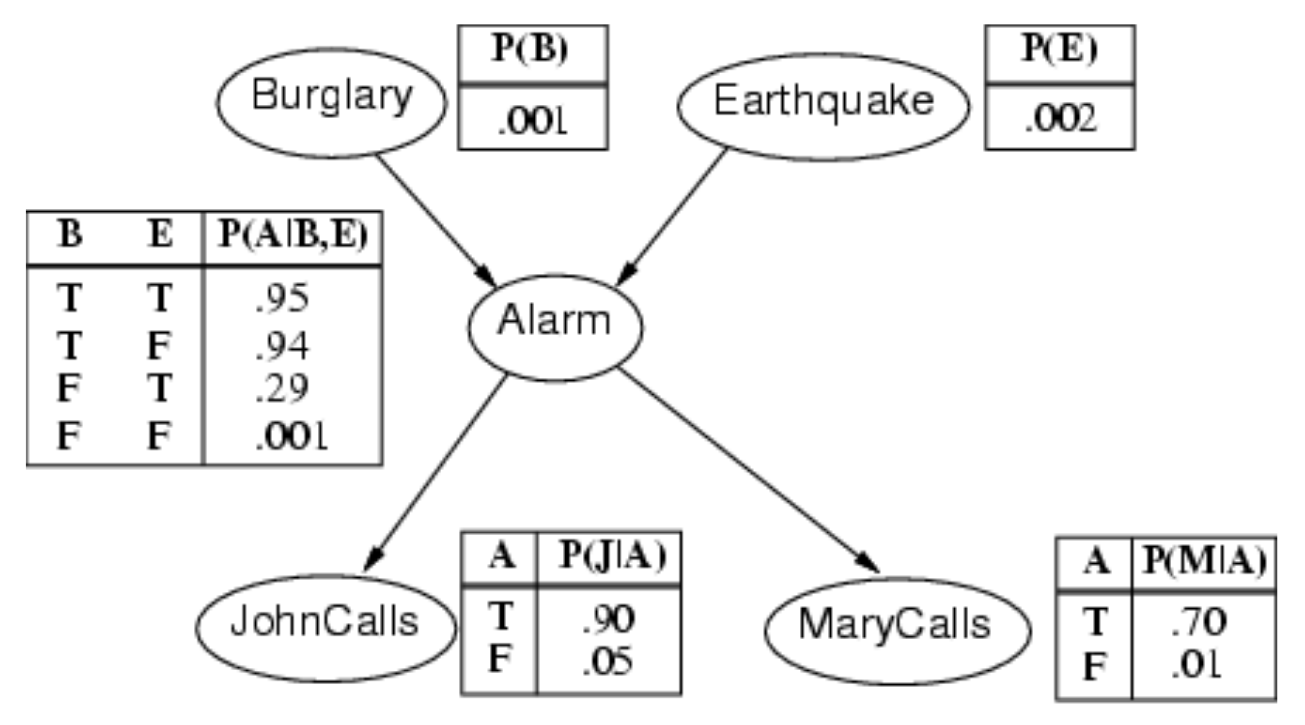
\includegraphics[width=0.7\textwidth]{cpt}
\caption{Rete bayesiana con CPTs}
\label{fig:cpt}
\end{figure}

\textbf{Nota}: le probabilità iniziali P(B) e P(E) sono le probabilità che B ed E si verifichino (siano veri). Per trovare le probabilità che B ed E siano falsi basta semplicemente fare il calcolo 1 - P(B) o 1 - P(E).\\

Una CPT per una variabile booleana $X_i$ con k genitori ha $2^k$ righe (date le combinazioni dei genitori). Con n variabili/nodi sono quindi richieste $n2^k$ righe

Nella rete bayesiana dell'esempio quante righe ci sono? Basta fare il conto: $1 (E) + 1 (B) + 2^2 (A) + 2^1 (J) + 2^1 (M) = 1 + 1 + 4 + 2 + 2 = 10$ righe.

Nella \textbf{full joint distribution} occorre tenere conto di tutte le combinazioni possibile. Nell'esempio ci sono 5 variabili, quindi $2^5 = 32$ numeri.

La full joint distribution viene definita come il prodotto delle distribuzioni di probabilità condizionata locali: 

\begin{equation}
 P(x_1, ..., x_n) = \prod_{i=1}^n P(X_i | Parents(X_i))
\end{equation}

Ad esempio si può calcolare la probabilità che l'allarme sia scattato e che sia John che Mary abbiano chiamato, ma non si siano verificati né un terremoto né un'intrusione:\\

$P(j \land m \land a \land \neg b \land \neg e) = P(j|a)P(m|a)P(a|\neg b, \neg e) P(\neg b) P(\neg e)$.\\

Svolgendo tutti i calcoli risulta che questa probabilità sia 0.000628 (molto bassa).

\subsection{Come costruire una rete Bayesiana?}

\begin{itemize}
 \item Scegliere un ordinamento delle variabili
 \item \texttt{for i = 1 to n do} aggiungi $X_i$ alla rete e scegli i suoi genitori in modo tale che $P(X_i | Parents(X_i)) = P(X_i| X_1, ..., X_{i-1})$
\end{itemize}
